\section*{\hypertarget{char}{Personajes}}
\addcontentsline{toc}{section}{Personajes}
%
"¡Soy EL Basch fon Ronsenburg!" \\
\indent -- Vaan
%
\begin{center} 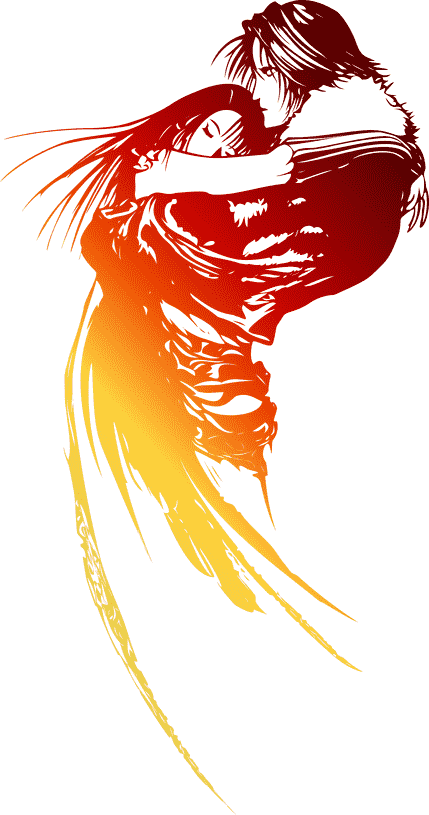
\includegraphics[width=0.9\columnwidth]{./art/images/ff8.png} \end{center}
%
Todos los jugadores juegan como uno de los aventureros del grupo de protagonistas. Se ponen en la piel de su personaje y hablan y actúan desde su perspectiva. El DJ también crea y asume el papel de muchos de los personajes no jugadores a lo largo de la aventura. Todos estos personajes habitan el mundo creado por el DJ, y lo definen a través de sus acciones y decisiones. Esta sección detalla diferentes aspectos que describen a un personaje. \subsubsection*{Creación de personajes}
Los personajes suelen tener distintas apariencias, personalidades, fortalezas y debilidades. Por lo tanto, las reglas de creación de personajes presentan muchas oportunidades para personalizar cómo sienten y juegan los personajes. La siguiente guía te dará las herramientas necesarias para crear tu personaje.
\pagebreak%

\begin{enumerate}[leftmargin=*]
	
\item Copia o imprime la \hyperlink{cs}{Hoja de personaje} que se incluye en la página siguiente. La hoja te ayuda a realizar un seguimiento de la información más importante sobre tu personaje, que puedes completar siguiendo esta guía. También hay un \hyperlink{csex}{ejemplo} de una hoja completa que puedes utilizar como guía para completar la tuya.

\vfill 

\item Elige el nombre de tu personaje y escribe una pequeña \textbf{Descripción} de él o ella. Para este punto también deberías hablar con el DJ para que puedas integrar mejor tu personaje al mundo del juego. Por ejemplo, si existen diferentes razas o tribus en el mundo, tu personaje puede formar parte de una de ellas.

\vfill	

\item Haz un pequeño resumen de la \textbf{Historia} de tu personaje hasta ahora y explica su motivación para unirse al grupo en esta aventura. Ten en cuenta que es muy probable que esta sea la primera aventura importante de tu personaje, por lo que probablemente no tenga una experiencia significativamente mayor que la de una persona promedio.

\vfill

\item Elige el \textbf{Talento} de tu personaje, que concede competencias especiales en habilidades que no son de combate. Lee la \mbox{\hyperlink{talent}{Subsección Talentos}} para obtener más detalles.

\vfill

\item Elige el \textbf{Oficio} que determina las competencias relacionadas con el combate. Normalmente, los personajes comienzan el juego en el Nivel 1, donde las habilidades y atributos iniciales están determinados por el oficio elegido. Lee la \hyperlink{job}{Subsección Oficios} para obtener más detalles.

\vfill

\item Según el oficio elegido, tu personaje se especializa en ciertas clases de armas y armaduras. Conversa con tu DJ sobre cuál sería el \textbf{Equipo} más lógico para tu personaje. Lee la \hyperlink{equip}{Subsección Equipo} para obtener más detalles.

\end{enumerate}

\vspace{1cm}

\example{Creación de Personaje}
{
Creamos un personaje llamado "Vaan", que es un niño humano rubio de 17 años de aspecto atlético. Vaan es un huérfano que sobrevive en la gran ciudad robándoles a los ciudadanos. A menudo actúa como figura paternal de otros huérfanos. Sueña con tener una aeronave y ser pirata de los cielos. En primer lugar, comprobamos con el DJ que Vaan encaja bien con el entorno dado y el resto del grupo. Luego, elegimos el talento \hyperlink{talent}{Líder} y el oficio \hyperlink{Thief}{Ladrón}, que parecen encajar mejor con Vaan. Con la tabla de atributos básicos del oficio determinamos los PV máximos de Vaan (20), Los PM máximos (14) y la AGI~(4). Todos los demás atributos comienzan en 0. También anotamos que conoce la técnica "Robar Gil". Finalmente, decidimos con el DJ si tiene sentido que nuestro ladrón pobre tenga un \hyperlink{mknife}{Cuchillo de Mithril}, Ropa y 100 Gil como equipo al iniciar la aventura.
}

\pagebreak
